\section{Strategic what-if: a fulfilment centre near Lisbon}\label{sec:network}

The frontier of \cref{sec:pareto} stops at about 92\% on-time delivery, and the plan map (\cref{fig:planmap}) shows where the missing points are.
Northern Portugal (the Porto sort centre) can only be served next-day from Asturias, a small site.
In practice most of that volume ships from Madrid on lanes that miss the overnight window.
This is a question for the network, not for daily operations, and the same machinery can answer it.

\paragraph{Experiment.}
We add a candidate FC in Azambuja, a logistics hub about 50\,km north-east of Lisbon, with 34 crews and 90 truck departures.
Its lanes to both Portuguese sort centres fit the overnight window.
The national inventory cover is unchanged and is re-spread over 11 FCs.
On each of the 31 test days, the day-ahead SP ($N=100$ true scenarios) is re-optimised for the base and the extended network, and both plans are evaluated on 1000 true scenarios.
Using the true distribution isolates the network effect from forecast error.
We report two prices of speed, because the business case depends on how much the next-day promise is worth.

\begin{table}[t]
\centering\small
\caption{Value of a fulfilment centre near Lisbon (31 test days). Savings are differences of expected daily cost (base minus extended network). ``Objective'' includes the price of speed $\lambda$, ``cost excl.\ late'' only out-of-pocket costs. The annualised figure is $365\times$ the regular-day mean, i.e.\ conservative (events excluded). Fixed costs of the site are not included: the annualised saving is the break-even annual cost of the site.}\label{tab:network}
\resizebox{\linewidth}{!}{\begin{tabular}{@{}rrrrrrrrr@{}}\toprule
$\lambda$ & \multicolumn{3}{c}{Daily saving, regular days (\EUR{})} & Saving, & On-time PT & On-time all & CO$_2$ (t/day) & Annualised \\
\cmidrule(lr){2-4}
 & objective & s.e. & cost excl. late & events & (\%) & (\%) & & (M\EUR{}/yr) \\ \midrule
1.0 & 50{,}142 & 1{,}648 & 25{,}496 & 141{,}941 & 53.6 $\to$ 92.6 & 91.61 $\to$ 96.89 & 202.4 $\to$ 182.9 & 18.30 \\
2.5 & 89{,}843 & 2{,}830 & 22{,}717 & 205{,}465 & 54.4 $\to$ 96.4 & 91.71 $\to$ 97.47 & 202.9 $\to$ 185.9 & 32.79 \\
\bottomrule\end{tabular}
}
\end{table}

\begin{figure}[t]
  \centering
  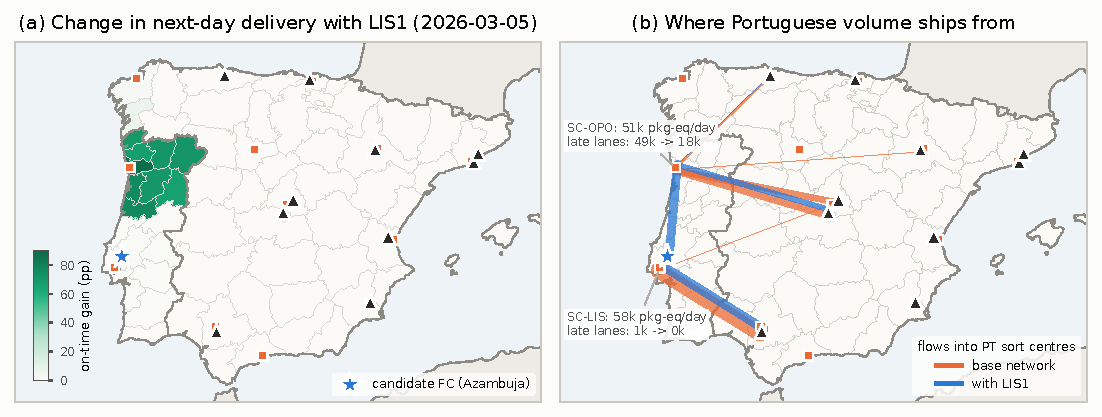
\includegraphics[width=\linewidth]{lisbon_map}
  \caption{(a) Gain in expected next-day delivery by district when the Lisbon FC is added (5 March 2026, $\lambda=1$): the Porto catchment gains 60--85 points; the Lisbon catchment, already served on time from Seville, is unchanged. (b) Expected package-equivalents flowing into the two Portuguese sort centres by origin FC, without (orange) and with (blue) the new site; line width is proportional to volume.}
  \label{fig:lisbonmap}
\end{figure}

\begin{figure}[t]
  \centering
  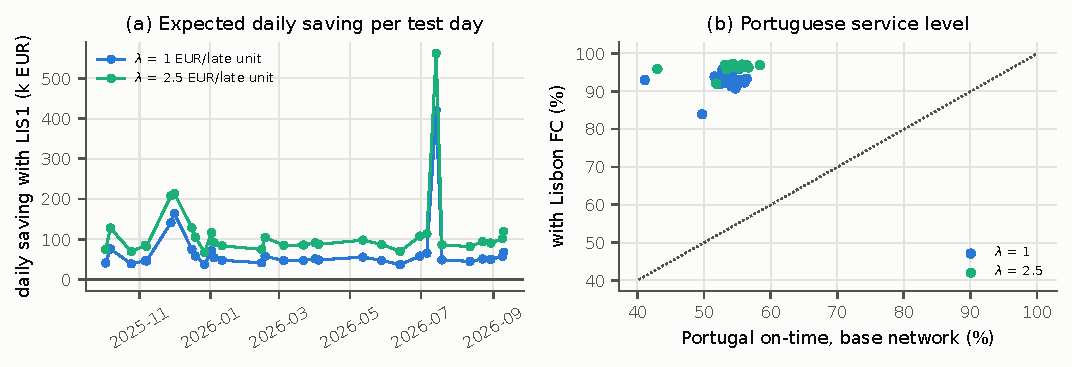
\includegraphics[width=\linewidth]{network_design}
  \caption{(a) Expected daily saving on every test day: the saving is positive on every day, and largest on peak days (Black Friday week, Prime Day), when the extra site also relieves capacity. (b) Portuguese on-time rate per test day, base vs.\ extended network.}
  \label{fig:networkdesign}
\end{figure}

\paragraph{Findings} (\cref{tab:network}, \cref{fig:lisbonmap,fig:networkdesign}).
\begin{itemize}
  \item \textbf{Service.} Next-day delivery in Portugal rises from 54\% to 93\% ($\lambda=1$), or to 96\% ($\lambda=2.5$). Network-wide it rises from 91.6\% to 96.9\%, and Spain is unaffected.
  \item \textbf{Cost.} On regular days, out-of-pocket operating cost falls by \EUR{25}k per day, through shorter lanes, fewer spot trucks and less overtime. Including the value of speed at $\lambda=1$, the saving is \EUR{50}k per day. The saving is positive on all 31 days (minimum \EUR{37}k) and peaks at \EUR{420}k on Prime Day 2026.
  \item \textbf{Emissions.} CO$_2$ falls by 19.5\,t per day (about 10\%), because Portuguese volume no longer crosses the peninsula.
  \item \textbf{Break-even.} The conservative annualised saving is \EUR{9.3}M per year in pure operating cost, and \EUR{18.3}M per year including the value of the next-day promise at \EUR{1} per unit. A site of this size pays off if its annual fixed cost (lease, overhead, depreciation) is below these figures.
\end{itemize}
Even with the new site, part of the Porto volume still ships late from Madrid: with unchanged national cover, the inventory positioned at Azambuja is the binding constraint.
That is a reminder that network design, inventory placement and capacity planning should eventually be optimised jointly (\cref{sec:discussion}).
